\documentclass[aps, pre, preprint, amsmath, amssymb]{revtex4}
\usepackage{braket}
\usepackage{graphicx}
\usepackage{amsfonts}
\usepackage{bm}
\usepackage{bbm}
\usepackage{lipsum}
\usepackage{mathtools}
\usepackage{color}
\usepackage{mathrsfs}
\usepackage{algorithm}
\usepackage{algpseudocode}

\usepackage[colorlinks=true,	bookmarks=true,
			linktocpage=true,	linkcolor=blue,  
            anchorcolor=blue,   urlcolor = red,
            citecolor=green]{hyperref}
\newcommand{\e}{\mathrm{e}}
\newcommand{\I}{\mathrm{i}}
\newcommand{\R}{\mathbb{R}}
\newcommand{\N}{\mathbb{N}}
\newcommand{\E}{\mathbb{E}}
\renewcommand{\d}{\mathrm{d}}
\renewcommand{\P}{\mathbb{P}}
\DeclareMathOperator{\sgn}{sgn}
\DeclareMathOperator{\diag}{diag}
\newcommand{\caputo}[1]{\prescript{C}{}{\partial_t^{#1}}}
\newcommand{\flaplace}[1]{\bm{\Delta}^{#1}}
\newcommand{\xiaokuo}[1]{\left(#1\right)}
\newcommand{\zhongkuo}[1]{\left[#1\right]}
\newcommand{\dakuo}[1]{\left\{#1\right\}}
\newcommand{\red}{\textcolor{red}}
\renewcommand{\algorithmicrequire}{\textbf{Input:}}
\renewcommand{\algorithmicensure}{\textbf{Output:}}
\makeatletter
\newenvironment{breakablealgorithm}
  {% \begin{breakablealgorithm}
   \begin{center}
     \refstepcounter{algorithm}% New algorithm
     \hrule height.8pt depth0pt \kern2pt% \@fs@pre for \@fs@ruled
     \renewcommand{\caption}[2][\relax]{% Make a new \caption
       {\raggedright\textbf{\ALG@name~\thealgorithm} ##2\par}%
       \ifx\relax##1\relax % #1 is \relax
         \addcontentsline{loa}{algorithm}{\protect\numberline{\thealgorithm}##2}%
       \else % #1 is not \relax
         \addcontentsline{loa}{algorithm}{\protect\numberline{\thealgorithm}##1}%
       \fi
       \kern2pt\hrule\kern2pt
     }
  }{% \end{breakablealgorithm}
     \kern2pt\hrule\relax% \@fs@post for \@fs@ruled
   \end{center}
  }
\makeatother

\begin{document}

\title[Stochastic Processes Classification by ResNet-50]{Stochastic Processes Classification by ResNet-50}
%
%\author{Weihua Deng}
%
%\address{School of Mathematics and Statistics, Gansu Key Laboratory of Applied Mathematics and Complex 
%Systems, Lanzhou University, Lanzhou, 730000, P.R. China}
%\email{dengwh@lzu.edu.cn}
\date{\today}

%\tableofcontents
%\begin{abstract}
%\end{abstract}
%\keywords{}
%\maketitle
\begin{itemize}
	\item alternating process with L\'{e}vy walk and Brownian motion;
	\item counting process: Poisson process;
	\item Gaussian process: Brownian motion and fractional Brownian motion;
	\item L\'{e}vy process: symmetric $\alpha$-stable process and $\beta$-stable subordinator;
	\item multiple internal states process: L\'{e}vy walk with multiple internal states and fractional compound Poisson process with multiple internal states;
	\item continuous-time random walks. 
\end{itemize}
%
\tableofcontents
%\maketitle
\appendix

\section{Models}
In this appendix, we present a brief introduction to the concepts of stochastic processes involved in this paper. 
We provide theoretical insights about the normal and anomalous diffusion models considered in this classification, as well as the description of the pseudocode used for simulations (see Appendix \ref{sub:codes}).
The Python and MATLAB implementations of all the algorithms described below are available at \url{https://github.com/tangxiangong/ClassTop/}.
\subsection{Stable distribution and power-law distribution}
Before introducing the diffusion models, let us take a look at the stable distribution \cite{mandelbrot1960pareto, applebaum2009levy, ken1999levy} and the power-law distribution.
Let $X_1$ and $X_2$ be independent copies of a random variable $X$. Then $X$ is said to be stable if for any positive constants $a$ and $b$ the random variable $aX_1+bX_2$ has the same distribution as $cX+d$ for some constants $c>0$ and $d$. 
Furthermore, a random variable $X$ is stable if and only if its characteristic function $\E\zhongkuo{\e^{\I kX}}$ can be written as \cite{klafter2011first, applebaum2009levy, ken1999levy}  
\begin{equation}
\varphi(k;\alpha, \beta, \mu, \sigma)=\exp\xiaokuo{-\sigma^{\alpha}|k|^{\alpha}\xiaokuo{1-\I\beta\omega(k;\alpha,\sigma)\sgn(k)}+\I\mu k}
\end{equation}
with 
\begin{equation}
\omega(k; \alpha, \sigma)=\left\{
\begin{array}{lll}
\xiaokuo{|\sigma k|^{1-\alpha}-1}\tan{\xiaokuo{\frac{\pi\alpha}{2}}}, &  &\alpha\neq 1,\\
-\frac{2}{\pi}\ln{|\sigma k|}, & & \alpha =1,
\end{array}
\right.
\end{equation}
where $\alpha\in (0,2]$, is the index of stability, $\beta\in [-1,1]$, called the skewness parameter, is a measure of asymmetry, $\mu\in\R$ is a shifted parameter, and $\sigma>0$ is called the scaling  parameter (without loss of generality, we will take $\sigma=1$ in the following text).

When $\mu=\beta=0$, it is called the symmetric $\alpha$-stable distribution, and when $\alpha < 1$ and $\beta=1$, it is called one-sided (or totally skewed) $\alpha$-stable distribution. In this paper, we take $\mu=0$ for totally skewed stable distribution, in this case, the distribution is supported by $[0,\infty)$.

When $\alpha=2$, the stable distribution is normal distribution.
If $\alpha<2$, the stable distribution is power-law, that is, the probability density function (PDF) of symmetric $\alpha$-stable distribution $L_{\alpha}(x)$, and the PDF of totally skewed $\alpha$-stable distribution $S_{\alpha}(t)$ have the following asymptotic formulae \cite{de1980simple}
\begin{equation}
	L_{\alpha}(x) \propto \frac{1}{|x|^{1+\alpha}}, 
	\quad |x|\to\infty,
\end{equation}
\begin{equation}
	S_{\alpha}(t) \propto \frac{1}{t^{1+\alpha}},
	\quad t\to\infty.
\end{equation}

To generate a symmetric $\alpha$-stable random variable $X$, we can first generate a random variable $V$ uniformly distributed on $(-\pi/2, \pi/2)$ and an exponential random variable $W$ with mean 1, and then compute $X$ as following \cite{janicki1994can, weron1995computer}
\begin{equation}\label{eq:alpha-rnd}
X = \frac{\sin{(\alpha V)}}{(\cos{V})^{1/\alpha}}
\cdot \xiaokuo{\frac{\cos{(V-\alpha V)}}{W}}^{(1-\alpha)/\alpha}.
\end{equation}
Similarly, we can get a totally skewed $\alpha$-stable $S$ as below \cite{janicki1994can, weron1995computer},
\begin{equation}\label{eq:beta-rnd}
S=c_1\frac{\sin{(\alpha(V+c_2))}}{(\cos{V})^{1/\alpha}}\cdot
\xiaokuo{\frac{\cos{(V-\alpha(V+c_2))}}{W}}^{(1-\alpha)/\alpha},
\end{equation}
where $c_1=(\cos{(\pi\alpha/2)})^{-1/\alpha}$ and $c_2=\pi/2$.

The simulation algorithms for symmetric and totally skewed stable distribution are Algorithm \ref{alg:alpha-rnd} and Algorithm \ref{alg:beta-rnd} respectively. In addition, one can also use the \textbf{Stable Distribution} in the MATLAB Statistic and Machine Learning Toolbox (\url{https://www.mathworks.com/help/stats/stable-distribution.html}) or \textbf{levy\_stable} in the Python package SciPy (\url{https://docs.scipy.org/doc/scipy/reference/generated/scipy.stats.levy_stable.html}) to generate random numbers of stable distribution.
\subsection{Continuous-time random walk}\label{sub:ctrw}
The continuous-time random walk (CTRW) model \cite{codling2008random, deng2020modeling, metzler2000random, klafter2011first} is based on the idea that the length of a given jump, as well as the waiting time elapsing between two successive jumps of a particle are drawn from a PDF $\psi(x, t)$. From $\phi(x, t)$, the jump length PDF $\lambda(x)$ and the waiting time PDF $\psi(t)$ can be deduced by marginal PDF. 
Here, we consider decoupled CTRW, that is, the waiting time and jump length are independent, $\phi(x, t)=\lambda(x)\psi(t)$.
If $x(t)$ denotes the position of particle with initial position $x(0)=0$, then 
\begin{equation}\label{eq:ctrw}
	x(t)=\sum_{k=1}^{N(t)}\xi_k
\end{equation}
with
\begin{equation}
	N(t)=\max\dakuo{n\in \N: \sum_{k=1}^n \tau_k \leqslant t},
\end{equation}
where waiting times $\dakuo{\tau_n}\overset{\textnormal{i.i.d}}{\sim} \psi(t)$ and jump lengths $\dakuo{\xi_n}\overset{\textnormal{i.i.d}}{\sim}\lambda(x)$.

Different types of CTRW processes can be categorised by the characteristic waiting time (mean-value of waiting time) and the jump length variance being finite or diverging\cite{metzler2000random}, respectively.
Therefore, we consider four cases of CTRW model. For finite and diverging characteristic waiting time, we choose exponential distribution and totally skewed $\beta$-stable distribution (power-law), respectively. 
For finite and diverging jump length variance, we choose symmetric $\alpha$-stable distribution with $\alpha < 2$ and normal distribution ($\alpha=2$), respectively.

For the finite characteristic waiting time and jump length variance CTRW model, it can model the normal diffusion in the sense of scaling limit with mean-squared displacement (MSD) $\langle x^2(t)\rangle\propto t$. 
For the finite characteristic waiting time and diverging jump length variance CTRW model, also called the L\'{e}vy flight, its MSD is diverging. But we can regard $\langle |x(t)|^{\delta}\rangle\propto t^{\delta/\alpha}$  as MSD for $0<\delta< \alpha \leqslant 2$ \cite{metzler2000random}.
For the diverging characteristic waiting and finite jump length variance CTRW model, its MSD $\langle x^2(t)\rangle\propto t^{\beta}$ \cite{metzler2000random}. 
However, the equations governing PDFs for these four situation have a unified form \cite{mandelbrot1960pareto,deng2020modeling, RN60, RN61, RN64, RN65}, as below,
\begin{equation}
\frac{\partial}{\partial t}P(x,t)=K\prescript{}{0}{D_t^{1-\beta}}\Delta^{\alpha/2}P(x,t),
\end{equation}
where $K$ is the generalized diffusion coefficient, $\prescript{}{0}{D_t^{1-\beta}}$ is the Riemann-Liouville fractional derivative operator \cite{bleanu2019handbook, sabatier2007advances, podlubny1998fractional} of oder $\beta\leqslant 1$, 
\begin{equation}
\prescript{}{0}{D_t^{1-\beta}}f(t)=\frac{\d}{\d t}\int_0^t\frac{(t-s)^{\beta-1}}{\Gamma(\beta)}f(s)\d s,
\end{equation}
and $\Delta^{\alpha/2}$ is the fractional Laplace operator \cite{lischke2020fractional,pozrikidis2018fractional}. 
Therein, $\beta=1$ corresponds to the exponential waiting time, and $\alpha=2$ corresponds to normal jump length.
Last, the simulation algorithm for these four CTRW models is given by Algorithm \ref{alg:ctrw}.

\begin{figure}[H]
\centering	
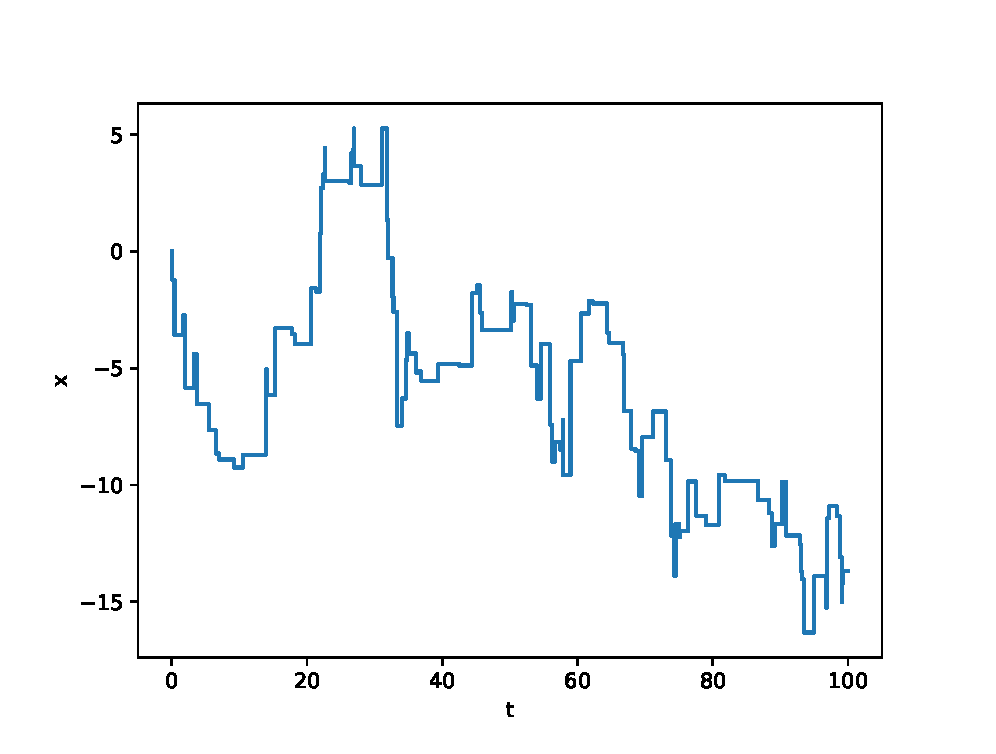
\includegraphics[scale=0.5]{figures/ctrw1}	
\caption{CTRW with finite characteristic waiting time and jump length variance}
\end{figure}
\begin{figure}[H]
\centering	
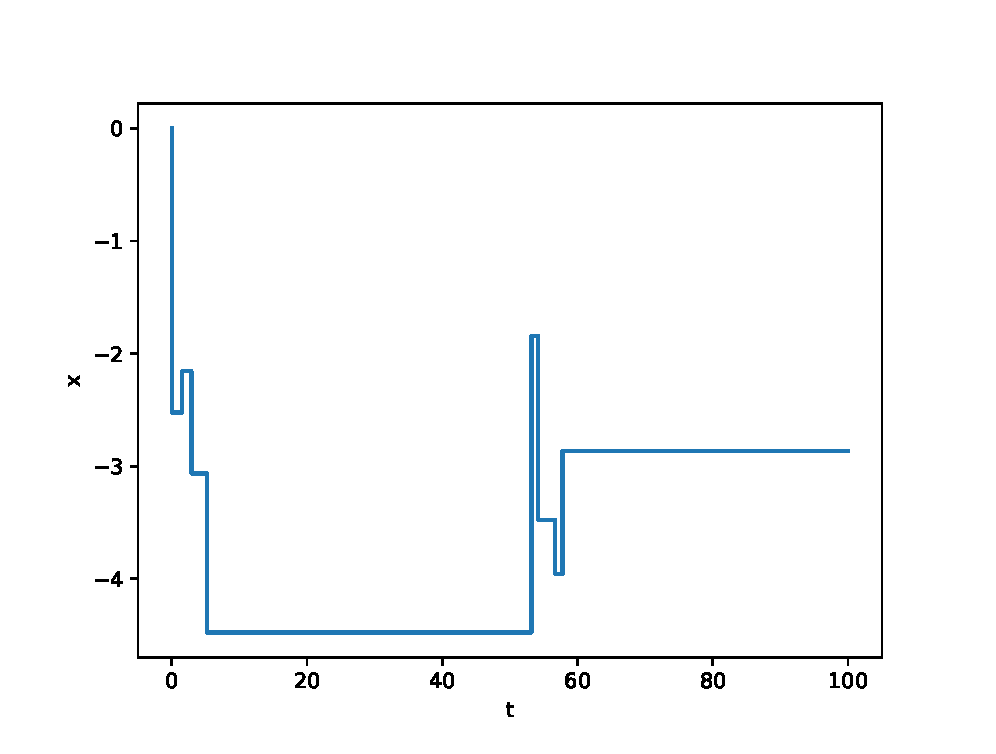
\includegraphics[scale=0.5]{figures/ctrw2}	
\caption{CTRW with diverging characteristic waiting time and finite jump length variance}
\end{figure}
\begin{figure}[H]
\centering	
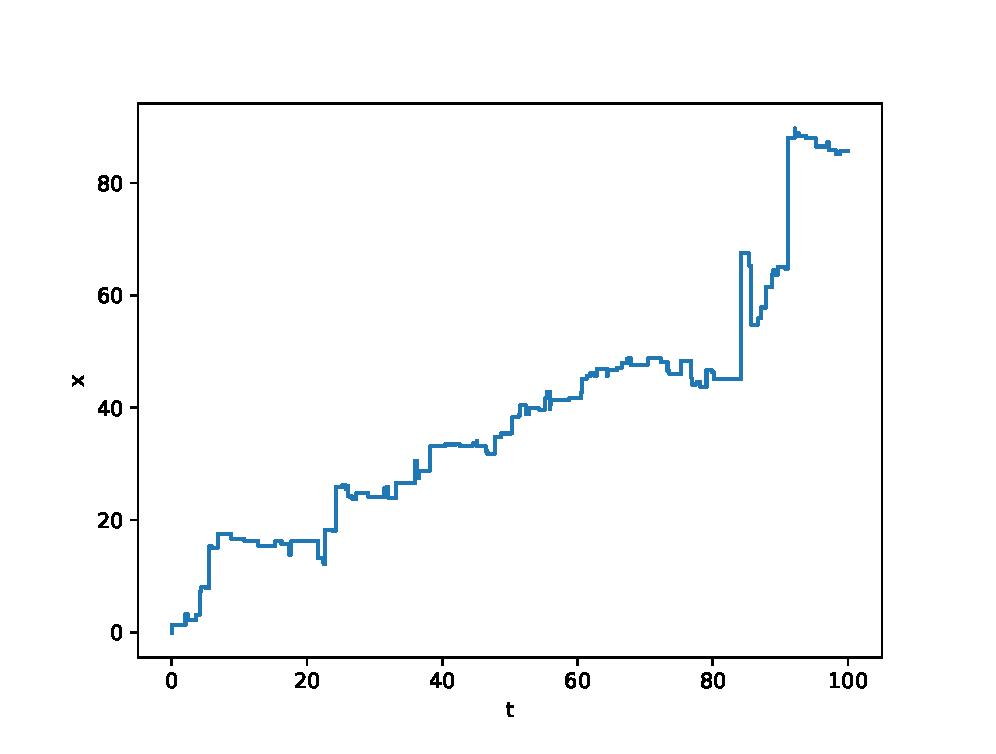
\includegraphics[scale=0.5]{figures/ctrw3}	
\caption{CTRW with finite characteristic waiting time and diverging jump length variance}
\end{figure}
\begin{figure}[H]
\centering	
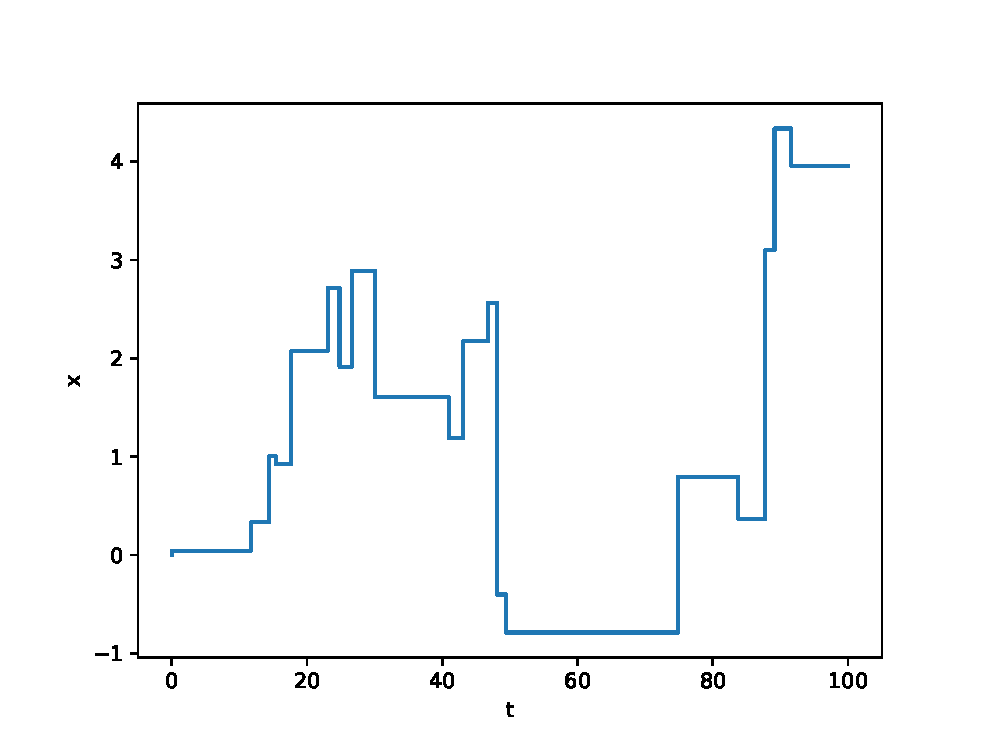
\includegraphics[scale=0.5]{figures/ctrw4}	
\caption{CTRW with diverging characteristic waiting time and jump length variance}
\end{figure}


\subsection{L\'{e}vy process}
Let $\bm{X}=\bm{X}(t, \omega)$ be a $d$-dimensional  stochastic process defined on a probability space $(\Omega, \mathscr{F}, \P)$.
We say that it has independent increments if for each $n\in \N$ and each $0\leqslant t_1 < t_2 < \cdots < t_{n+1} < \infty$ the random variables $\{\bm{X}(t_{j+1})-\bm{X}(t_j):1\leqslant j \leqslant n\}$ are independent and that it has stationary increments if each $\bm{X}(t_{j+1})-\bm{X}(t_j)\overset{\textnormal{d}}{=}\bm{X}(t_{j+1}-t_j)-\bm{X}(0)$, where the symbol $\overset{\textnormal{d}}{=}$ denotes identical distribution. 
Then $\bm{X}$ is a L\'{e}vy process \cite{ken1999levy, applebaum2009levy} if
\begin{enumerate}
	\item $\bm{X}(0)=0$, a.s.;
	\item $\bm{X}$ has independent and stationary increments;
	\item $\bm{X}$ is stochastically continuous, i.e., for all $a>0$ and  for all $t\geqslant 0$ 
	\begin{equation*}
		\lim_{s\to t}\P\xiaokuo{\left|\bm{X}(t)-\bm{X}(s)\right|>a}=0.
	\end{equation*}
\end{enumerate}
Because of its property of independent increments, L\'{e}vy process is Markovian.

According to L\'{e}vy-khintchine theorem \cite{mainardi2008origin, ken1999levy, applebaum2009levy}, we know that the characteristic function of L\'{e}vy process $\bm{X}$ has the following formula
\begin{equation}
\E\zhongkuo{\e^{\I \bm{k}\cdot\bm{X}(t)}}=\e^{t\phi(\bm{k})},
\end{equation}
\begin{equation}
\phi(\bm{k})=\I\bm{b}\cdot\bm{k}-\frac{1}{2}\bm{k}\cdot\bm{Ak}+\int_{\R^d\backslash\dakuo{0}}\xiaokuo{\e^{\I\bm{k}\cdot\bm{y}}-1-\I\bm{k}\cdot\bm{y}\mathbbm{1}_{\dakuo{|\bm{x}|<1}}(\bm{y})}\nu(\d\bm{y}),
\end{equation}
where $\bm{b}$ is a vector in $\R^d$, $\bm{A}$ is a $d\times d$ real symmetric semi-positive definite matrix, $\mathbbm{1}$ is the indicator function of  set, and $\nu$ is a L\'{e}vy measure, satisfying 
\begin{equation}
	\int_{\R^d\backslash\dakuo{0}}\min{\dakuo{1, |\bm{y}|^2}}\nu(\d\bm{y})<\infty.
\end{equation}

\subsubsection{isotropic $\alpha$-stable L\'{e}vy process}
We say L\'{e}vy process $\bm{L}_{\alpha}(t)$ is isotropic $\alpha$-stable if for any fixed $t\geqslant 0$, $\bm{L}_{\alpha}(t)$ is an isotropic stable random vector with index of stability $0<\alpha\leqslant 2$. 
And its characteristic function has the following specific formula 
\begin{equation}\label{eq:alpha-stable}
\E\zhongkuo{\e^{\I\bm{k}\cdot\bm{L}_{\alpha}(t)}}=\e^{-\sigma^{\alpha}|\bm{k}|^{\alpha}t},
\end{equation}
where $\sigma >0$ is the scaling parameter. 

According to \eqref{eq:alpha-stable}, we can obtain that the PDF $P(\bm{x},t)$ of $\bm{L}_{\alpha}(t)$ satisfies following equation
\begin{equation}
	\frac{\partial}{\partial t}P(\bm{x},t)={\Delta}^{\alpha/2}P(\bm{x}, t),
\end{equation}
Here, we focus on the one-dimensional isotropic (or symmetric) $\alpha$-stable L\'{e}vy process.

When $\alpha=2$, the one-dimensional stable L\'{e}vy process ${L}_{\alpha}(t)$ is the Brownian motion ${B}(t)$. 
Brownian motion $B(t)$ is the only continuous L\'{e}vy process, and is also a Gaussian process with mean $\E\zhongkuo{B(t)}=0$ and covariance $\E\zhongkuo{B(s)B(t)}=2\min\dakuo{t, s}$ for $t, s \geqslant 0$. 
And the PDF of $B(t)$ is
\begin{equation}
P(x,t)=\frac{1}{\sqrt{4\pi t}}\exp{\dakuo{-\frac{x^2}{4t}}}.
\end{equation}

The algorithm used to simulate one-dimensional $\alpha$-stable L\'{e}vy process trajectories is described in Algorithm \ref{alg:stable}.
Here, we use the equation 
\begin{equation}\label{eq:euler1}
	L_{\alpha}(t_{n+1})=L_{\alpha}(t_n)+(t_{n+1}-t_n)^{1/\alpha}\xi_n
\end{equation}
to simulate trajectories, where $\dakuo{\xi_n}$ are independent random variables of symmetric $\alpha$-stable distribution.

\subsubsection{$\beta$-stable subordinator}
A subordinator \cite{applebaum2009levy,ken1999levy} is a one-dimensional L\'{e}vy process that is non-decreasing (a.s.). 
And subordinator $T(t)$ is a $\beta$-stable subordinator if for any fixed $t\geqslant 0$, $T(t)$ is a totally skewed $\beta$-stable random variable with index of stability $0<\beta<1$. 
The Laplace transform of $T(t)$ is given by \cite{applebaum2009levy}
\begin{equation}
\E\zhongkuo{\e^{-\lambda T(t)}}=\e^{-\lambda^{\beta}t}.
\end{equation}
According to above Laplace transform, one can get the PDF $P(T, t)$ of $T(t)$ satisfies
\begin{equation}
{\partial_t}P(T, t)=-\partial_T^{\beta}P(T, t)-\frac{T^{-\beta}}{\Gamma(1-\beta)},
\end{equation}
where $\partial_t^{\beta}$ is the Caputo fractional derivative operator \cite{bleanu2019handbook,pozrikidis2018fractional} of order $\beta<1$,
\begin{equation}
\partial_t^{\beta}u(x,t)=\frac{1}{\Gamma(1-\beta)}\int_0^t(t-s)^{-\beta}\partial_s u(x, s)\d s.
\end{equation}

Similar to equation \eqref{eq:euler1}, we use equation 
\begin{equation}\label{eq:euler2}
T(t_{n+1})=T(t_n)+(t_{n+1}-t_n)^{1/\beta}\zeta_n 
\end{equation}
to simulate the trajectories of $\beta$-stable subordinator, where $\dakuo{\zeta_n}$ are independent random variables of totally skewed $\beta$-stable distribution. The simulation algorithm is Algorithm \ref{alg:subordinator}.

\subsubsection{Poisson process}
The (time homogeneous) Poisson process of intensity $\lambda >0$ is a L\'{e}vy process $N(t)$ taking values in $\N$, and
\begin{equation}
	\P\zhongkuo{N(t)=n}=\frac{(\lambda t)^n}{n!}\e^{-\lambda t}
\end{equation}
for each $n=0$, $1$, $2$, $\cdots$. 
The probability distribution $P(n, t)=\P\zhongkuo{N(t)=n}$ satisfies following equation
\begin{equation}
\frac{\partial}{\partial t}P(n, t)=\lambda\xiaokuo{P(n,t)-P(n-1,t)}.
\end{equation}

According to the properties of independent and stationary increments, the Poisson process can also be defined by stating that the time differences between events of the counting process are exponential variables with mean $1/\lambda$. So we can use independent random numbers of mean-$1/\lambda$ exponential distribution with  $\dakuo{\pi_n}$ to simulate Poisson process's trajectories, that is, 
\begin{equation}\label{eq:poisson}
	N(t_n)=n,\; t_n = t_{n-1} + \pi_n,\; t_0 = 0.
\end{equation}
The simulation algorithm is Algorithm \ref{alg:Poisson}.
\begin{figure}[H]
\centering
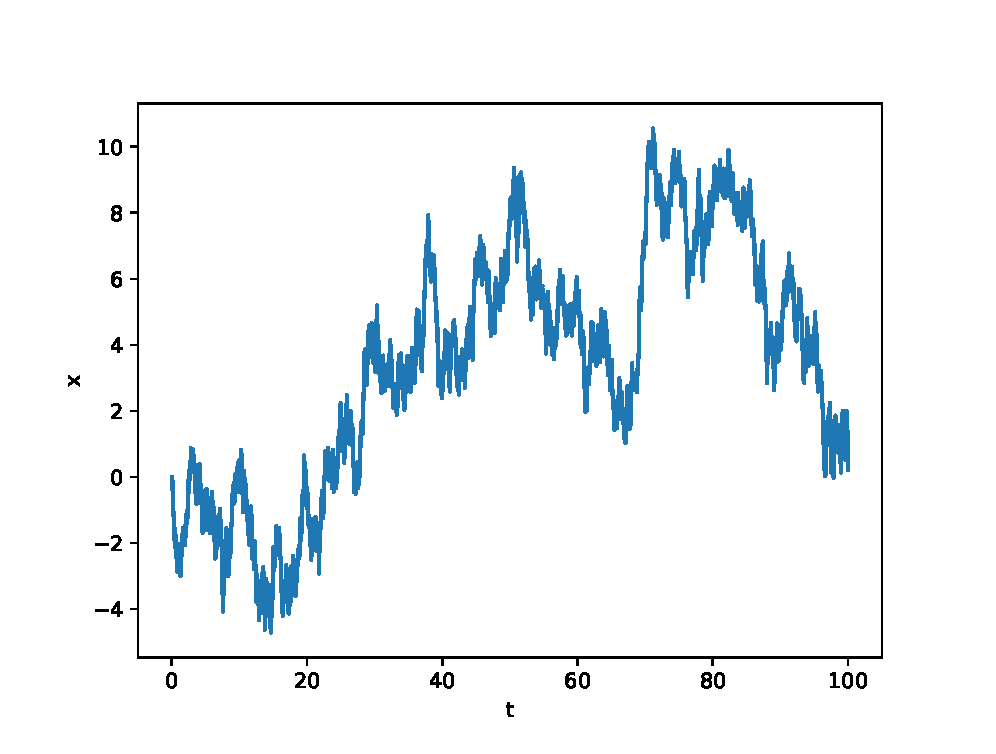
\includegraphics[scale=0.5]{figures/brown}
\caption{Brownian motion}
\end{figure}
\begin{figure}[H]
\centering
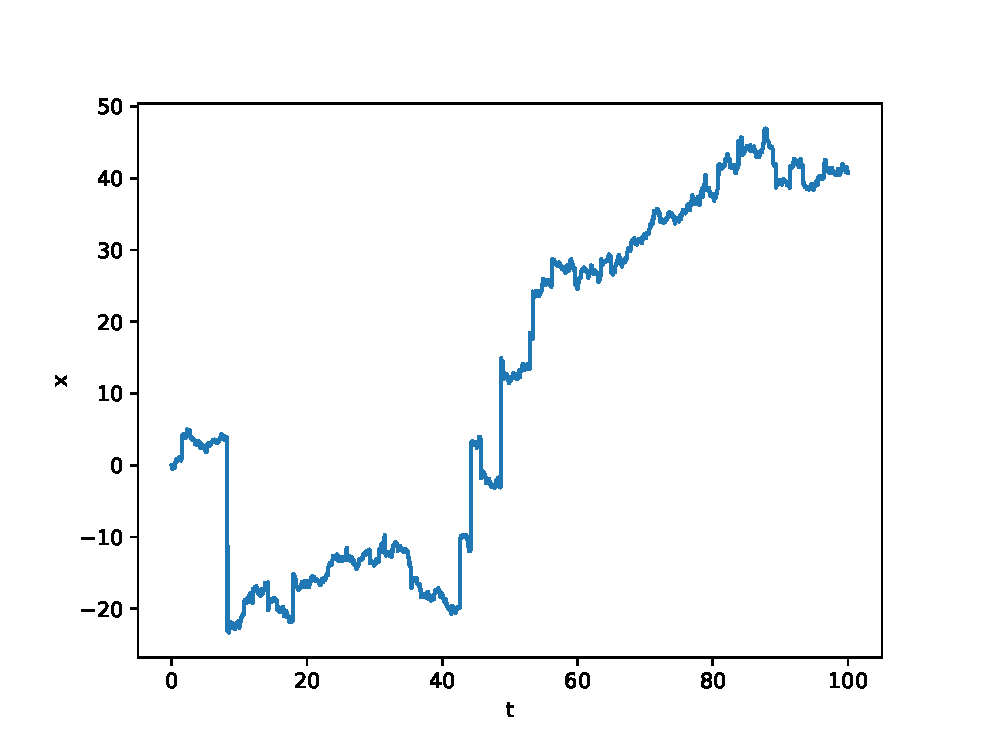
\includegraphics[scale=0.5]{figures/levy}
\caption{$\alpha$-stable L\'{e}vy process with $\alpha<2$}
\end{figure}
\begin{figure}[H]
\centering
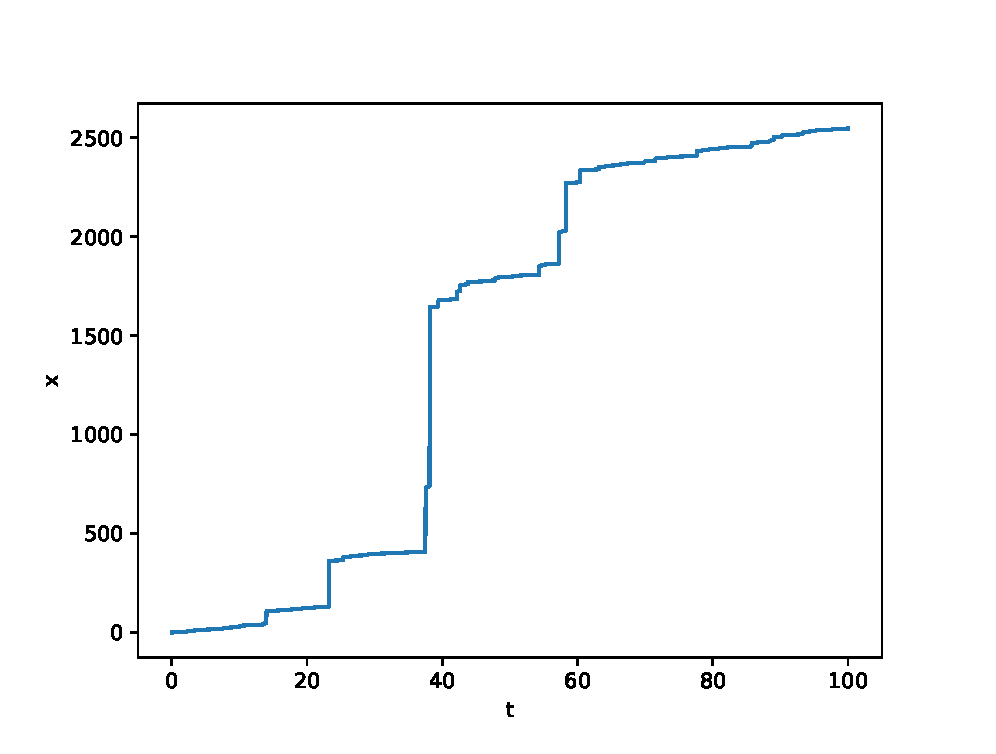
\includegraphics[scale=0.5]{figures/subordinator}
\caption{stable subordinator}
\end{figure}
\begin{figure}[H]
\centering
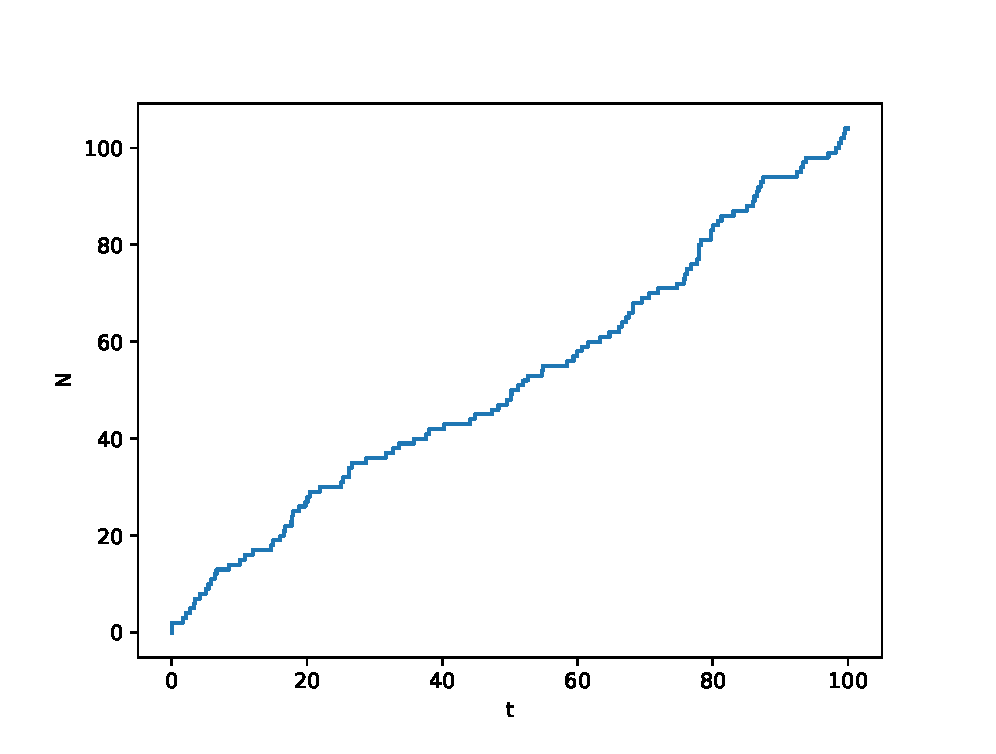
\includegraphics[scale=0.5]{figures/poisson}
\caption{Poisson process}
\end{figure}

\subsection{Fractional Brownian motion}
Fractional Brownian motion \cite{decreusefond1999stochastic, dieker2004simulation, rogers1997arbitrage, biagini2008stochastic, mandelbrot1960pareto} $B_{H}(t)$ with Hurst index $0<H<1$ is a Gaussian process with stationary increments, and satisfies following properties: 
\begin{equation}
	B_{H}(0)=0, \textnormal{\;a.s.},
\end{equation}
\begin{equation}
	\E\zhongkuo{B_{H}(t)}=0
\end{equation}
for all $t\geqslant 0$,
and
\begin{equation}
	\E\zhongkuo{B_{H}(t)B_{H}(s)}=\frac{1}{2}\xiaokuo{t^{2H}+s^{2H}-|t-s|^{2H}}
\end{equation}
for each $t$, $s\geqslant 0$. 
The mathematical definition of fractional Brownian motion is given by Mandelbrot and Ness \cite{mandelbrot1960pareto}, as following stochastic integral of Brownian motion $B(t)$
\begin{equation}
B_{H}(t)=\frac{1}{\Gamma(H+1/2)}\int_{\R}\zhongkuo{\xiaokuo{t-s}_{+}^{H-1/2}-\xiaokuo{-s}_{+}^{H-1/2}}\d B(s),
\end{equation}
where $x_{+}=\max\dakuo{x, 0}$. Specially, $B_{1/2}(t)=B(t)$. In addition, in reference \cite{huy2003remark}, the author proved that fractional Brownian motion is not Markov unless $H=1/2$.

The mean-squared displacement of $B_{H}(t)$ is $\E\zhongkuo{\xiaokuo{B_H(t)}^2}=t^{2H}$, so when $H<1/2$, it is a subdiffusion, when $H>1/2$, it is a superdiffusion. 
Since $B_{H}(t)$ is a Gaussian process, its characteristic function can be easily obtained by its mean and covariance, 
\begin{equation}
\E\zhongkuo{\e^{\I kB_{H}(t)}}=\exp{\dakuo{-\frac{1}{2}|k|^2t^{2H}}}.
\end{equation}
Denote $P(x,t)$ as the PDF of $B_{H}(t)$. 
Then we can get 
\begin{equation}
P(x,t)=\frac{1}{\sqrt{2\pi t^{2H}}}\exp{\dakuo{-\frac{x^2}{2t^{2H}}}},
\end{equation}
and
\begin{equation}
\frac{\partial}{\partial t}P(x,t)=Ht^{2H-1}\frac{\partial^2}{\partial x^2}P(x,t).
\end{equation}
%In ref.{sss}, the authors proved $B_{H}(t)$ is not Markovian when $H\neq 1/2$.

Various numerical approaches have been proposed to simulate fractional Brownian motion exactly. Here we use the Davies-Harte method \cite{davies1987tests, dieker2004simulation} and the Hosking method \cite{hosking1984modeling, dieker2004simulation} via the \textit{stochastic} Python package (\url{https://pypi.org/project/stochastic/}). Details about the numerical implementations can be found in the associated references.
\begin{figure}[H]
\centering
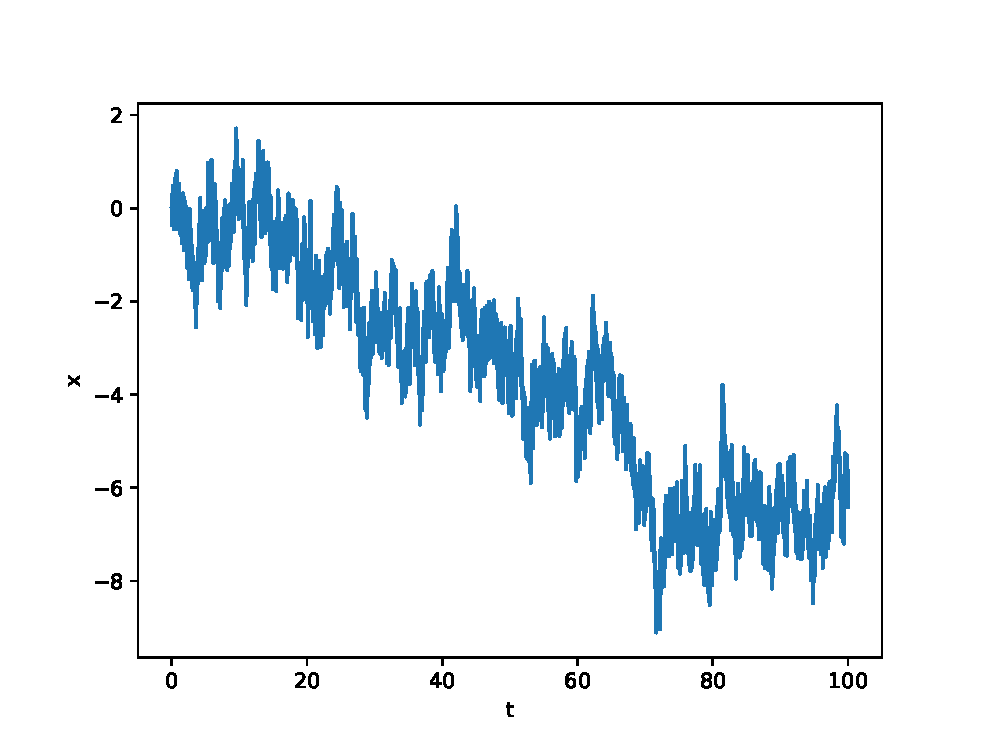
\includegraphics[scale=0.5]{figures/fbm1}
\caption{fractional Brownian motion with Hurst index $H<1/2$}
\end{figure}
\begin{figure}[H]
\centering
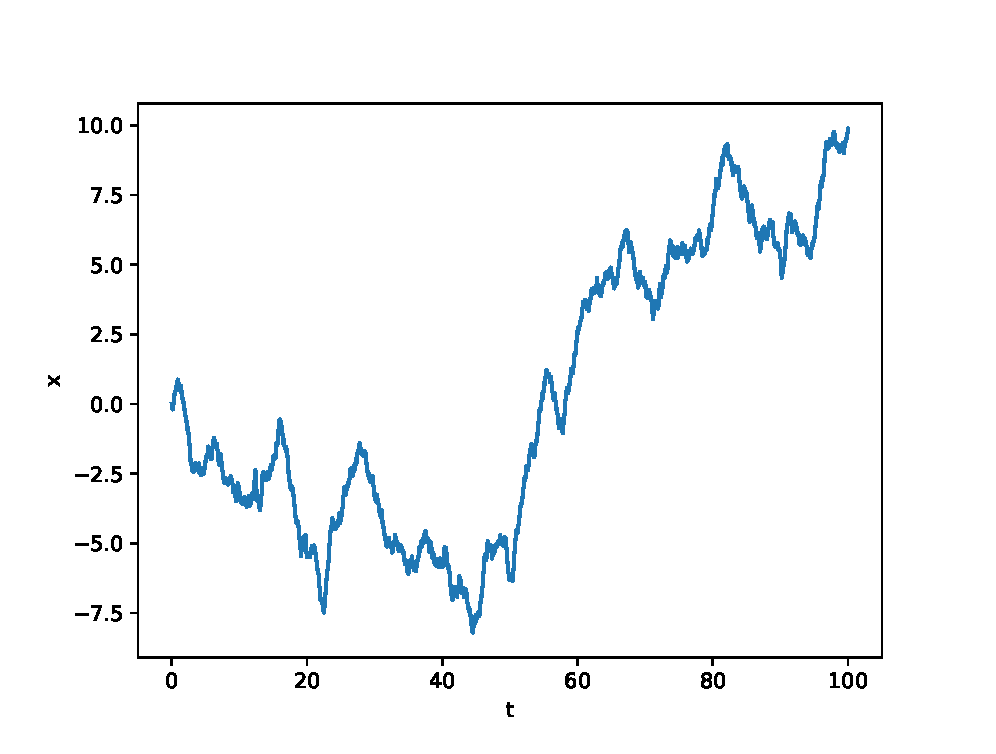
\includegraphics[scale=0.5]{figures/fbm2}
\caption{fractional Brownian motion with Hurst index $H>1/2$}
\end{figure}

\subsection{Alternating process}
A two-state process \cite{wang2019aging} serves as an intermittent search process, which alternates between L\'{e}vy walk \cite{2015, wang2019levy} and Brownian motion \cite{benichou2005optimal,lomholt2008levy}, i.e., L\'{e}vy walk $\longrightarrow$ Brownian motion $\longrightarrow$ L\'{e}vy walk $\longrightarrow \cdots$.
The searcher displays a slow active motion in the Brownian phase, during which the hidden target can be detected. 
While in L\'{e}vy walk phase, the searcher aims to relocate into some unvisited region to reduce oversampling. 
This kind of intermittent search process has wide applications in physical or biological problems \cite{bell2012searching, song2018neuronal}.

The sojourn time distributions of the two-state process switching between L\'{e}vy walk and
Brownian phase are $\psi^{+}(t)$ and $\psi^{-}(t)$, respectively. The
subscripts '+' and '-' are introduced to represent the
L\'{e}vy walk and Brownian phase, respectively. This process can be explicitly described by means of the velocity
process $v(t)$ which also consists of two states: $v^{+}(t)$ for
L\'{e}vy walk and $v^{-}(t)$ for Brownian motion. The PDF of $v^{+}(t)$ is $\delta(|v|-v_0)/2$ for some constant velocity $v_0$, whereas $v^{-}(t)=\sqrt{2}\xi(t)$ with $\xi(t)$ being Gaussian white noise.

Let the sojourn time distributions in the two states be a power-law form with exponents $\alpha_{\pm}$, that is, 
\begin{equation}
\psi_{\pm}(t) \propto t^{-(1+\alpha_{\pm})}
\end{equation}
for large $t$. For $\alpha_{\pm}\in (0,1)$, we know that one-sided $\alpha_{\pm}$-stable distribution has the above power-law form, so we can use equation \eqref{eq:beta-rnd} to get such a random variable.
In addition, we can assume $\psi_{\pm}(t)$ has the following expression
\begin{equation}
\psi_{\pm}(t)=\left\{
\begin{array}{lll}
C(t+1)^{-(1+\alpha_{\pm})}, & & t\geqslant 0, \\
0, & & t<0.
\end{array}
\right.
\end{equation}
By using the normalized property of the probability density function, one can get the parameter $C=\alpha_{\pm}$. 
Hence, the probability distribution function 
\begin{equation}
\Psi_{\pm}(t)=\left\{
\begin{array}{lll}
1-\xiaokuo{t+1}^{-\alpha_{\pm}}, & & t\geqslant 0, \\
0, & & t<0.
\end{array}
\right.	
\end{equation}
Therefore, if random variable $\xi\sim \Psi_{\pm}(t)$, then 
\begin{equation}\label{eq:power-rnd}
\xi = (1-X)^{-1/\alpha_{\pm}}-1,
\end{equation}
where $X$ is a random variable uniformly distributed on $(0,1)$.

The MSD of this two-state process has the following expression \cite{wang2019aging}
\begin{equation}
\langle x^2(t)\rangle \sim K_1t^{\nu_1}+K_2t^{\nu_2},
\end{equation}
where $K_1$ and $K_2$ are constants, the values $\nu_1$ and $\nu_2$ are given in the following table.
\begin{table}[H]
\centering
\caption{Parameters' values}
\begin{tabular}{|c|l|l|}
\hline
Specific cases & $\nu_1$ & $\nu_2$ \\
\hline
$\alpha_{+}=\alpha_{-}<1$ & $2$ & $1$ \\
\hline 
$1<\alpha_{\pm}<2$ &$3-\alpha_{+}$ &$1$ \\
\hline
$\alpha_{+}<\alpha_{-}<1$&$2$&$\alpha_{+}-\alpha_{-}+1$\\
\hline
$\alpha_{+}<1<\alpha_{-}<2$ & $2$ &$\alpha_{+}$ \\
\hline
$\alpha_{-}<\alpha_{+}<1$ & $\alpha_{-}-\alpha_{+}+2$ & $1$ \\
\hline
$\alpha_{-}<1<\alpha_{+}<2$ & $\alpha_{-}-\alpha_{+}+2$ & $1$\\
\hline
\end{tabular}
\end{table}
\begin{figure}[H]
\centering
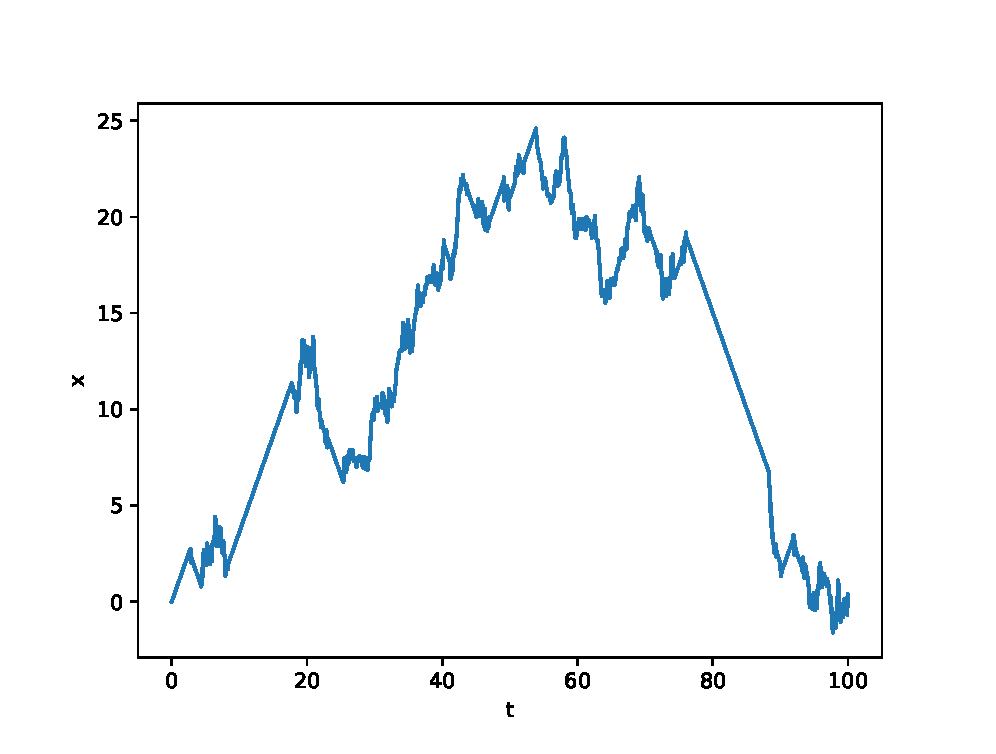
\includegraphics[scale=0.5]{figures/alter}
\caption{alternating process with L\'{e}vy walk and Brownian motion}
\end{figure}

\subsection{Multiple internal states process}

\subsubsection{fractional compound Poisson process with multiple internal states}\label{sub:fcp}
Fractional Poisson process is a renewal process whose probability PDF of the holding/waiting times between two subsequent events has the asymptotic behavior $\phi(\tau)\sim 1/\tau^{1+\alpha}$, $0<\alpha<1$ when time is long enough. 
Let $N(t)$ be the fractional Poisson process, i.e., there exist independent identically distributed random variables $\dakuo{\tau_n}\sim \phi(\tau)$ with $\phi(\tau) \sim 1/\tau^{1+\alpha}$ for $0<\alpha<1$ and large $\tau$,
and $\dakuo{\xi_n}$ a sequence of independent identically distributed variables (jump lengths). Then $X(t)=\sum\limits_{n=1}^{N(t)}\xi_n$ is the fractional compound Poisson process. 

Therefore, when the waiting time distribution is power-law with exponent $0<\alpha<1$, CTRW model \eqref{eq:ctrw} is a fractional compound Poisson process. 
Furthermore, we can generalize the renewal processes to have multiple internal states, where the waiting times for different internal states are drawn from different distribution. 
Here, we focus on fractional compound Poisson process $X(t)$ with multiple internal states \cite{RN67}, that is, $N(t)$ of $X(t)$ is a fractional Poisson process with multiple internal states. Each internal state has an own distribution of holding time, but the distribution of the jump lengths are all simply taken as normal distribution. 
In other words, $X(t)$ is a kind of CTRW process with multiple internal states whose characteristic waiting time is diverging and jump length variance is finite.  

Suppose that $X(t)$ has $N$ internal states. The transition of the internal states is described by a Markov chain with transition matrix $M\in \R^{N\times N}$.  
And the element $M_{ij}$ of $M$ represents the transition probability from state $i$ to state $j$.
Here, the bras $\bra{\cdot}$ and kets $\ket{\cdot}$ denote the row and column vectors respectively.
Let $\Phi(t)=\diag{\xiaokuo{\phi^{(1)}(t), \phi^{(2)}(t), \cdots, \phi^{(N)}(t)}}$ be the waiting time distribution matrix and $\Lambda(x)=\diag{\xiaokuo{\lambda^{(1)}(x), \lambda^{(2)}(x), \cdots, \lambda^{(N)}(x)}}$ be the jump length one.
And we use the notation $\ket{\textnormal{init}}$ to represent the column vector of initial distribution of the internal states.
In the Laplace space, $\widehat{\Phi}(s)\sim I-\Phi^*(s)$ where $\Phi^*(s)=\diag{\xiaokuo{B_{\alpha_1}s^{\alpha_1}, \cdots, B_{\alpha_N}s^{\alpha_N}}}$, $0<\alpha_1, \cdots, \alpha_N < 1$.
Then the Fokker-Planck equation for $X(t)$ is  \cite{RN67}
\begin{equation}
\begin{aligned}
M^{T}\frac{\partial}{\partial t}\ket{G({x}, t)}=&
(M^T-I)\diag{\xiaokuo{B_{\alpha_1}^{-1}, \cdots, B_{\alpha_N}^{-1}}}\diag{\xiaokuo{D_t^{1-\alpha_1}, \cdots, D_t^{1-\alpha_N}}}\ket{G(x, t)}\\
&+ M^T\diag{\xiaokuo{K_{\alpha_1}, \cdots, K_{\alpha_N}}}\diag{\xiaokuo{D_t^{1-\alpha_1}, \cdots, D_t^{1-\alpha_N}}}\Delta\ket{G(x, t)},
\end{aligned}
\end{equation}
where $\ket{G(x,t)}$ is the PDF of $X(t)$, $\dakuo{K_{\alpha_i}}_{i=1}^N$ are generalized diffusion coefficient, $\dakuo{D_t^{1-\alpha_i}}_{i=1}^N$ are Riemann-Liouville fractional derivative operator.

As for renewal process $N(t)$ of fractional compound Poisson process $X(t)$, after each update, a Markov chain is used to determine which internal state it is in. 
Therefore, we should know how to generate a non-uniform discrete distributed random number.

Suppose that $Y$ is a finite discrete random variable taking values in $\dakuo{1,2,\cdots, N}$, and 
$\P\zhongkuo{Y=j}=p_j$, $j=1,2,\cdots, N$.
Here we use the inverse transform method to sample $Y$.
The probability distribution function of $Y$ is 
\begin{equation}
F_{Y}(x) = \left\{
\begin{array}{lll}
0, & & x<1 \\
\sum\limits_{k=1}^{j}p_k, & & j\leqslant x < j+1, \; j=1,\cdots, N-1, \\
1, & & x\geqslant N.
\end{array}
\right.
\end{equation}
The inverse of $F_{Y}$ can be written as 
\begin{equation}
F^{-1}_{Y}(u) = j, \;\textnormal{if } \sum_{k=1}^{j-1}p_k<u\leqslant\sum_{k=1}^jp_k, \; j=1, \cdots, N.
\end{equation}
If $U$ is a random variable uniformly distributed on $(0,1)$, then $F^{-1}_Y(U)$ is identically distributed with $Y$.
Therefore, we can generate a sample $\xi$ of $U$, then $F_{Y}^{-1}(\xi)$ is a sample of $Y$. 
The pseudocode is Algorithm \ref{alg:finite}.

After generating a sample of $Y$, we now can generate the trajectories of fractional compound Poisson process with multiple internal states $X(t)$.
Firstly, we should determine the initial state by the initial distribution $\ket{\textnormal{init}}$. 
In fact, we can choose initial state by generating a sample $I$ of probability distribution $\P\zhongkuo{Y=j}=\ket{\textnormal{init}}_{j}$. 
Then the initial state is the $I$-th state. Next, after update in $m$-th internal state, we can generate a sample $n$ of probability distribution $\P\zhongkuo{Y=j}=M_{mj}$ to determine that next update is occurred is in the $n$-th internal state. The details is given by Algorithm \ref{alg:fcp}.

\begin{figure}[H]
\centering
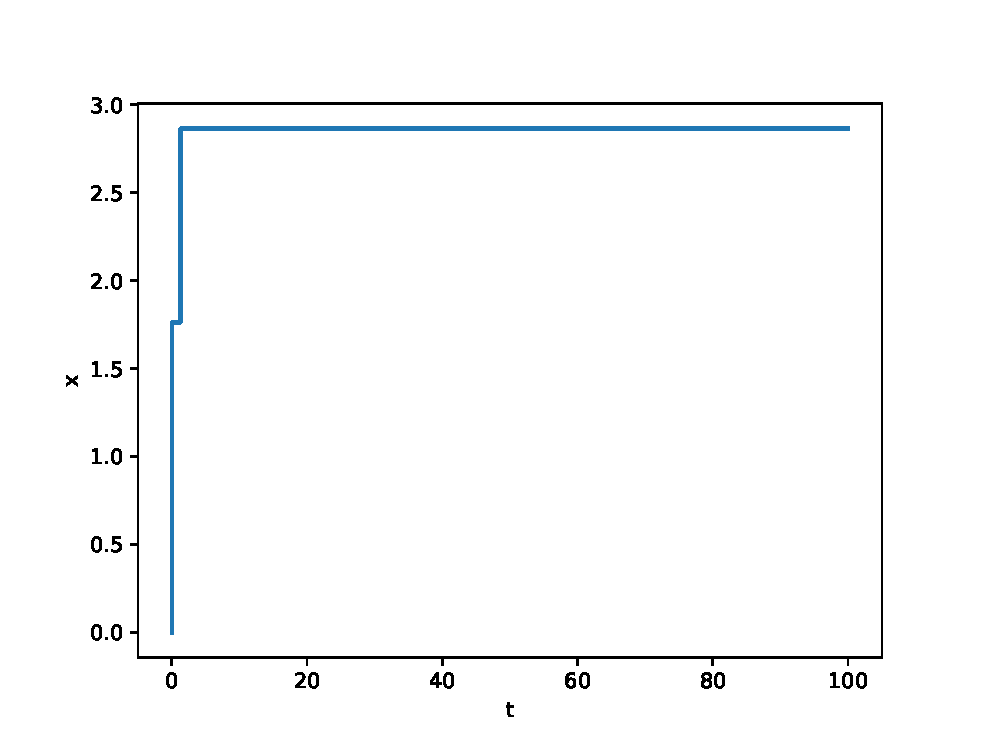
\includegraphics[scale=0.5]{figures/fcp}
\caption{fractional compound Poisson process with multiple internal states}
\end{figure}


\subsubsection{L\'{e}vy walks with multiple internal states}
As mentioned in Appendix \ref{sub:ctrw}, the L\'{e}vy flight has divergent MSD and the particle's jump does not cost any time \cite{metzler2000random}. In order to make the model fitter for the real natural phenomena, L\'{e}vy walk is used to describe superdiffusion properly and naturally \cite{2015,shlesinger1986levy}. The linearly-coupled L\'{e}vy walk with constant velocity $v_0$ is one of the most representative and important kinds of L\'{e}vy walks.
Comparing to waiting time in CTRW, L\'{e}vy walk is given a random variable $\tau$ representing the duration of each step, and the total distance of each step of the particle’s movement for linearly-coupled L\'{e}vy walk is then $v_0\tau$.

The L\'{e}vy walk with multiple internal states \cite{xu2018levy} is similar with fractional compound Poisson process with multiple internal states. The meanings of  initial distribution vector $\ket{\textnormal{init}}$ and the transition matrix $M$ are same to the ones in Appendix \ref{sub:fcp}. However, the distributions of sojourn times $\dakuo{\phi_n(t)}$ need not to be power-law, they can also be exponential. In addition, compared to fractional compound Poisson process with multiple internal states, L\'{e}vy walk with multiple internal states removes the jump length distribution, but has an additional feature, distributions of speed $\dakuo{\lambda_n(v_0)}$. In Appendix \ref{sub:codes}, we propose an algorithm (Algorithm \ref{alg:lw}) to simulate the trajectories of L\'{e}vy walk with multiple internal states.
\begin{figure}[H]
\centering
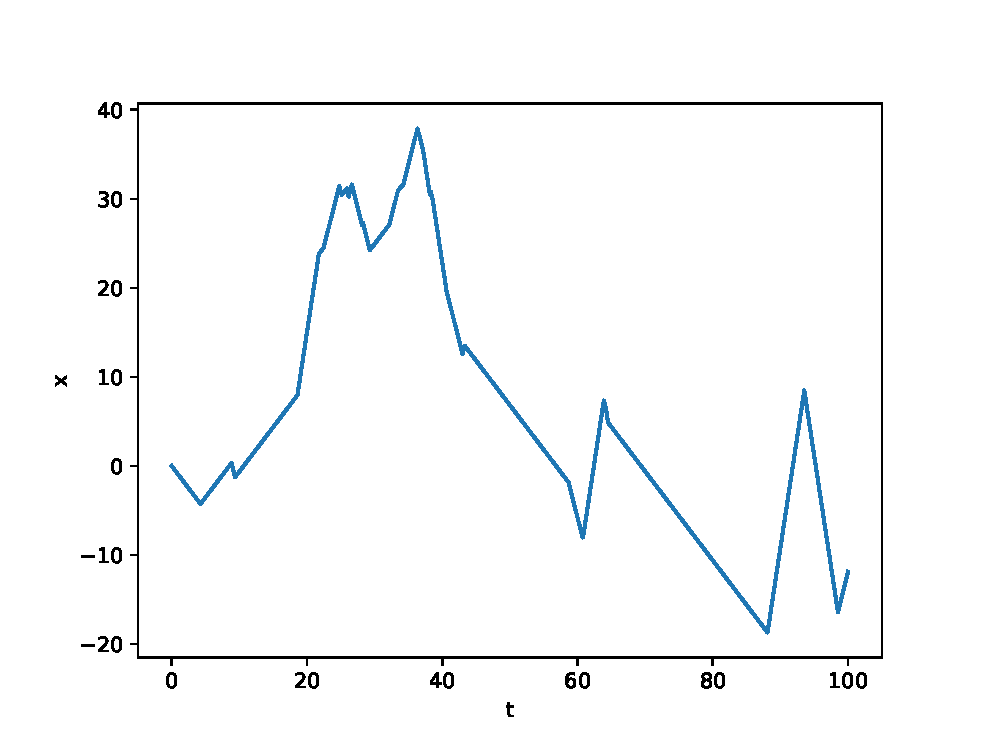
\includegraphics[scale=0.5]{figures/lw}
\caption{L\'evy walk with multiple internal states}
\end{figure}

\section{Pseudocodes}\label{sub:codes}
\subsection{Random number generator}

\begin{breakablealgorithm}
\caption{Generating finite discrete distribution random number}
\label{alg:finite}
\begin{algorithmic}[1]
\Require probability vector $\bm{p}=(p_1,\cdots, p_N)$\Comment{$\P\zhongkuo{Y=j}=p_j$}
\Ensure a sample $y$ of $Y$
\State Compute the cumulative sum $\bm{q}=(q_1,\cdots,q_N)$ of $\bm{p}$ 
\State $q_0\gets 0$
\State Generate a sample $\xi$ uniformly distributed on $(0,1)$
\For{$k\gets 1$ to $N$}
\If{$q_{k-1}<\xi\leqslant q_{k}$}
\State $y=k$
\State \textbf{break}
\EndIf
\EndFor
\State\Return $y$
\end{algorithmic}
\end{breakablealgorithm}

~\\

\begin{breakablealgorithm}
\caption{Generating symmetric $\alpha$-stable random number}
\label{alg:alpha-rnd}
\begin{algorithmic}[1]
\Require index of stability $\alpha$
\Ensure symmetric $\alpha$-stable random number $\xi$
\State Generate a random number $V$ uniformly distributed on $(-\pi/2,\pi/2)$ and an exponential random number $W$ with mean 1
\State $\xi\gets\frac{\sin{(\alpha V)}}{(\cos{V})^{1/\alpha}}
\cdot \xiaokuo{\frac{\cos{(V-\alpha V)}}{W}}^{(1-\alpha)/\alpha}$\Comment{Equation \eqref{eq:alpha-rnd}}
\State\Return $\xi$
\end{algorithmic}
\end{breakablealgorithm}

~\\

\begin{breakablealgorithm}
	\caption{Generating totally skewed $\alpha$-stable random number}
	\label{alg:beta-rnd}
	\begin{algorithmic}[1]
		\Require index of stability $\alpha$
		\Ensure totally skewed $\alpha$-stable random number $\xi$
		\State{Generate a random number $V$ uniformly distributed on $(-\pi/2,\pi/2)$ and an exponential random number $W$ with mean 1}
		\State{$c_1 \gets (\cos{(\pi\alpha/2)})^{-1/\alpha}$ and $c_2\gets \pi/2$}
		\State{$\xi\gets c_1\frac{\sin{(\alpha(V+c_2))}}{(\cos{V})^{1/\alpha}}\cdot
\xiaokuo{\frac{\cos{(V-\alpha(V+c_2))}}{W}}^{(1-\alpha)/\alpha}$}\Comment{Equation \eqref{eq:beta-rnd}}
\State\Return $\xi$
\end{algorithmic}
\end{breakablealgorithm}

~\\

\begin{breakablealgorithm}
\caption{Generating power-law random number}
\label{alg:power-law}
\begin{algorithmic}[1]
\Require the exponent of power-law distribution $\alpha$
\Ensure power-law random number $\xi$
\State Generate a random number $X$ uniformly distributed on $(0,1)$
\State $\xi\gets (1-X)^{-1/\alpha}-1$\Comment{Equation \eqref{eq:power-rnd}}
\State \Return $\xi$
\end{algorithmic}
\end{breakablealgorithm}
\subsection{CTRW}
\begin{breakablealgorithm}
\caption{Generating CTRW trajectory}
\label{alg:ctrw}
\begin{algorithmic}[1]
\Require length of trajectory $T$, index of waiting time $\beta$ and index of jump length $\alpha$, and initial position $x_0$
\begin{Comment}
{$\beta=1$ means that the waiting time distribution is exponential}
\end{Comment}
\Ensure time vector $\bm{t}$ and position vector $\bm{x}$
\If{$\beta=1$}
\State Set \textit{random} as the random number generator of exponential distribution
\Else
\State Set \textit{random} as the random number generator of totally skewed $\beta$-stable distribution\Comment{Algorithm \ref{alg:beta-rnd}}
\EndIf
\State Generate empty vectors $\bm{t}$ and $\bm{x}$\Comment{Variable-length vectors}
\State $\bm{t}(1)\gets 0$ and $\bm{x}(1)\gets x_0$ \Comment{Initial value}
\State $t_{tot}\gets 0$\Comment{Total time}
\State $x_c\gets x_0$\Comment{Current position}
\State $n\gets 1$\Comment{Counter}
\While{\textbf{true}}
\State Generate a random number $\tau_n$ by generator \textit{random}
\If{$t_{tot}+\tau_n > T$}
\State $\bm{t}(n+1)\gets T$
\State $\bm{x}(n+1)\gets x_c$
\State \textbf{break}
\Else
\State $t_{tot}\gets t_{tot}+\tau_n$
\State $\bm{t}(n+1)\gets t_{tot}$
\State Generate a random number $\xi_n$ of symmetric $\alpha$-stable distribution \Comment{Algorithm \ref{alg:alpha-rnd}}
\State $x_c\gets x_c+\xi_n$ 
\State $\bm{x}(n+1)\gets x_c$
\State $n\gets n+1$
\EndIf
\EndWhile
\State\Return $\bm{t}$ and $\bm{x}$
\end{algorithmic}	
\end{breakablealgorithm}

\subsection{L\'{e}vy process}
\begin{breakablealgorithm}
	\caption{Generating $\alpha$-stable L\'{e}vy process trajectory}
	\label{alg:stable}
	\begin{algorithmic}[1]
		\Require {length of the trajectory $T$, index of stability $\alpha$ and time-stepping size $\tau$, and initial position $x_0$}
		\Ensure {time vector $\bm{t}$ and position vector $\bm{x}$}
		\State{$N \gets \lceil T/\tau\rceil$}
		\State{Generate empty vectors $\bm{t}$ and $\bm{x}$ of length $N+1$}
		\State{$\bm{t}(n)\gets (n-1)\tau$ for $n=1$, $\cdots$, $N+1$}
		\State{$\bm{x}(1)\gets x_0$}\Comment{Initial position}
		\State{$x_c \gets x_0$}\Comment{Current position}
		\State{Generate $N$ random numbers of symmetric $\alpha$-stable distribution $\dakuo{\xi_n}_{n=1}^N$}\Comment{Algorithm \ref{alg:alpha-rnd}}
		\For{$n\gets 1$ to $N$}
		\State{$x_c\gets x_c + \tau^{1/\beta}\xi_n$}
		\State{$\bm{x}(n+1)\gets x_c$}\Comment{Equation \eqref{eq:euler1}}
		\EndFor
		\State\Return $\bm{t}$ and $\bm{x}$
	\end{algorithmic}
\end{breakablealgorithm}

~\\

\begin{breakablealgorithm}
	\caption{Generating $\beta$-stable subordinator trajectory}
	\label{alg:subordinator}
	\begin{algorithmic}[1]
		\Require {length of the trajectory $T$, index of stability $\beta$ and time-stepping size $\tau$}
		\Ensure {time vector $\bm{t}$ and position vector $\bm{x}$}
		\State{$N \gets \lceil T/\tau\rceil $}
		\State{Generate empty vectors $\bm{t}$ and $\bm{x}$ of length $N+1$}
		\State{$\bm{t}(n)\gets (n-1)\tau$ for $n=1$, $\cdots$, $N+1$}
		\State{$\bm{x}(1)\gets 0$}\Comment{Initial value}
		\State{$x_c\gets 0$}\Comment{Current position}
		\State{Generate $N$ random numbers of totally skewed $\beta$-stable distribution $\dakuo{\zeta_n}_{n=1}^N$}\Comment{Algorithm \ref{alg:beta-rnd}}		
		\For{$n\gets 1$ to $N$}
		\State{$x_c\gets x_c + \tau^{1/\alpha}\zeta_n$}
		\State{$\bm{x}(n+1)\gets x_c$}\Comment{Equation \eqref{eq:euler2}}
		\EndFor
		\State\Return $\bm{t}$ and $\bm{x}$
	\end{algorithmic}
\end{breakablealgorithm}

~\\

\begin{breakablealgorithm}
	\caption{Generating Poisson process trajectory}
	\label{alg:Poisson}
	\begin{algorithmic}[1]
		\Require length of the trajectory $T$ and intensity $\lambda$
		\Ensure time vector $\bm{t}$ and position vector $\bm{x}$
		\State Generate empty vectors $\bm{t}$ and $\bm{x}$\Comment{Variable-length vectors}
		\State $\bm{t}(1)\gets 0$ and $\bm{x}(1)\gets 0$ \Comment{Initial value}
		\State $t_{tot}\gets 0$\Comment{Total time}
		\State $x_c\gets 0$\Comment{Current position}
		\State $n\gets 1$\Comment{Counter}
		\While{\textbf{true}}
		\State Generate a random number $\tau_n$ of exponential distribution with mean $1/\lambda$
		\If{$t_{tot}+\tau_n > T$}
		\State $\bm{t}(n+1)\gets T$
		\State $\bm{x}(n+1)\gets x_c$
		\State \textbf{break}
		\Else
		\State $t_{tot}\gets t_{tot}+\tau_n$
		\State $x_c \gets x_c + 1$
		\State $\bm{t}(n+1)\gets t_{tot}$
		\State $\bm{x}(n+1)\gets x_c$ 
		\State $n\gets n+1$
		\EndIf
		\EndWhile
		\State\Return $\bm{t}$ and $\bm{x}$
	\end{algorithmic}
\end{breakablealgorithm}

\subsection{Alternating process}
\begin{breakablealgorithm}
\caption{Generating alternating process trajectory}
\label{alg:alter}
\begin{algorithmic}[1]
\Require length of trajectory $T$, sojourn time distributions' exponents $\alpha_{+}$ and $\alpha_{-}$, velocity of L\'{e}vy walk $v_0$ and initial position $x_0$
\Ensure time vector $\bm{t}$ and position vector $\bm{x}$
\State Generate empty vectors $\bm{t}$ and $\bm{x}$\Comment{Variable vectors}
\State $\bm{t}(1)\gets 0$ and $\bm{x}(1)\gets x_0$\Comment{Initial position}
\State $t_{tot}\gets 0$\Comment{Total time}
\State $x_{c}\gets x_0$\Comment{Current position}
\State $n\gets 1$ \Comment{Counter}
\While{\textbf{true}}
\State Generate a random number $\xi_n$ uniformly distributed on $(0,1)$
\If{$\xi_n < 0.5$}
\State $d \gets -1$\Comment{Direction of L\'{e}vy walk}
\Else
\State $d\gets 1$
\EndIf
\State Generate a power-law random number $\tau_{n+}$ with exponent $\alpha_{+}$\Comment{Algorithm \ref{alg:power-law}}
\If{$t_{tot}+\tau_{n+}\geqslant T$}
\State $\bm{t}\gets (\bm{t}, T)$
\State $x_{c}\gets x_{c}+dv_0(T-t_{tot})$
\State $\bm{x}\gets (\bm{x}, x_{c})$
\State \textbf{break}
\Else
\State $t_{tot}\gets t_{tot}+\tau_{n+}$
\State $\bm{t}\gets (\bm{t}, t_{tot})$
\State $x_{c} \gets x_{c} + dv_0\tau_{n+}$
\State $\bm{x}\gets (\bm{x}, x_{c})$
\EndIf
\State Generate a power-law random number $\tau_{n-}$ with exponent $\alpha_{-}$\Comment{Algorithm \ref{alg:power-law}}
\If{$t_{tot}+\tau_{n-}\geqslant T$}
\State Generate a Brownian motion trajectory $\hat{\bm{t}}_{n-}$ and $\hat{\bm{x}}_{n-}$ with length $T-t_{tot}$ and initial position $x_{c}$\Comment{Algorithm \ref{alg:stable}}
\State $\bm{t}_{n-}\gets t_{tot}+\hat{\bm{t}}_{n-}(2:\textbf{end})$
\State $\bm{t}\gets (\bm{t}, \bm{t}_{n-})$

\State $\bm{x}\gets (\bm{x}, \hat{\bm{x}}_{n-}(2:\textbf{end}))$
\State \textbf{break}
\Else
\State Generate a Brownian motion trajectory $\tilde{\bm{t}}_{n-}$ and $\tilde{\bm{x}}_{n-}$ with length $\tau_{n-}$ and initial position $x_{c}$\Comment{Algorithm \ref{alg:stable}}
\State $\bm{t}_{n-}\gets t_{tot}+\tilde{\bm{t}}_{n-}(2:\textbf{end})$
\State $\bm{t}\gets (\bm{t}, \bm{t}_{n-})$
\State $\bm{x}\gets (\bm{x}, \hat{\bm{x}}_{n-}(2:\textbf{end}))$
\State $t_{tot}\gets t_{tot} + \tau_{n-}$
\State $x_{cur}\gets \bm{x}(\textbf{end})$
\EndIf
\State $n\gets n+1$
\EndWhile
\State\Return $\bm{t}$ and $\bm{x}$
\end{algorithmic}
\end{breakablealgorithm}

\subsection{Multiple internal states process}
\begin{breakablealgorithm}
\caption{Generating fractional compound Poisson process with multiple internal states trajectory}
\label{alg:fcp}
\begin{algorithmic}[1]
\Require length of trajectory $T$, index vector of waiting times $\bm{\alpha}=(\alpha_1,\cdots, \alpha_N)$, transition matrix $M$, initial state $\bm{I}=(I_1,\cdots, I_N)$  and initial position $x_0$
\Ensure time vector $\bm{t}$ and position vector $\bm{x}$
\State Set \textit{random} as the random number generator of totally skewed stable distribution\Comment{Algorithm \ref{alg:beta-rnd}}
\State Generate empty vectors $\bm{t}$ and $\bm{x}$\Comment{Variable-length vectors}
\State $\bm{t}(1)\gets 0$ and $\bm{x}(1)\gets x_0$ \Comment{Initial value}
\State $t_{tot}\gets 0$\Comment{Total time}
\State $x_c\gets x_0$\Comment{Current position}
\State $n\gets 1$\Comment{Counter}
\State Generate a sample $init$ of probability distribution $\P[Y=j]=I_j$\Comment{Algorithm \ref{alg:finite}}
\State $num_S \gets init$
\While{\textbf{true}}
\State Generate a random number $\tau_n$ by \textit{random} with parameter $\alpha_{num_S}$
\If{$t_{tot}+\tau_n > T$}
\State $\bm{t}(n+1)\gets T$
\State $\bm{x}(n+1)\gets x_c$
\State \textbf{break}
\Else
\State $t_{tot}\gets t_{tot}+\tau_n$
\State $\bm{t}(n+1)\gets t_{tot}$
\State Generate a random number $\xi_n$ of standard normal distribution
\State $x_c\gets x_c + \xi_n$
\State $\bm{x}(n+1)\gets x_c$ 
\State Generate a sample $num_{next}$ of probability distribution $\P[Y=j]=M_{num_S, j}$
\State $num_S \gets num_{next}$
\State $n\gets n+1$
\EndIf
\EndWhile
\State\Return $\bm{t}$ and $\bm{x}$
\end{algorithmic}	
\end{breakablealgorithm}

~\\

\begin{breakablealgorithm}
\caption{Generating L\'{e}vy walk with multiple internal states trajectory}
\label{alg:lw}
\begin{algorithmic}[1]
\Require length of trajectory $T$, vector of sojourn time distributions $\bm{w}=({w_1}(t),\cdots, w_N(t))$, vector of velocity distributions $\bm{v}(x) =(v_1(x), \cdots, v_N(x))$, transition matrix $M$, initial state $\bm{I}=(I_1, \cdots, I_N)$ and initial position $x_0$
\Ensure time vector $\bm{t}$ and position vector $\bm{x}$
\State Generate empty vectors $\bm{t}$ and $\bm{x}$\Comment{Variable-length vectors}
\State $\bm{t}(1)\gets 0$ and $\bm{x}(1)\gets x_0$ \Comment{Initial value}
\State $t_{tot}\gets 0$\Comment{Total time}
\State $x_c\gets x_0$\Comment{Current position}
\State $n\gets 1$\Comment{Counter}
\State Generate a sample $init$ of probability distribution $\P[Y=j]=I_j$\Comment{Algorithm \ref{alg:finite}}
\State $num_S \gets init$
\While{\textbf{true}}
\State Generate a random number $\tau_n$ of distribution $w_{num_S}(t)$
\State Generate a sample $\zeta_n$ uniformly distributed on $(0,1)$
\If{$\zeta_n < 0.5$}
\State $d\gets -1$
\Else
\State $d\gets 1$
\EndIf
\State Generate a random number $v_{0n}$ of distribution $v_{num_S}(x)$
\If{$t_{tot}+\tau_n > T$}
\State $\bm{t}(n+1)\gets T$
\State $x_c \gets x_c + dv_{0n}(T-t_{tot})$
\State $\bm{x}(n+1)\gets x_c$
\State \textbf{break}
\Else
\State $t_{tot}\gets t_{tot}+\tau_n$
\State $x_c \gets x_c + dv_{0n}\tau_n$
\State $\bm{t}(n+1)\gets t_{tot}$
\State $\bm{x}(n+1)\gets x_c$ 
\State Generate a sample $num_{next}$ of probability distribution $\P[Y=j]=M_{num_S, j}$
\State $num_S \gets num_{next}$
\State $n\gets n+1$
\EndIf
\EndWhile
\State\Return $\bm{t}$ and $\bm{x}$
\end{algorithmic}	
\end{breakablealgorithm}
\nocite{*}
\bibliographystyle{plain}
\bibliography{ref}

\end{document}